This part of ParTI is based on two core abstractions:
\begin{enumerate}
	\item Inherent trade-offs between traits that are evolutionarily important to increase performance in different objectives, drive variation in a population to distribute along a Pareto front.
	\item The Pareto front in trait-space is the hypervolume of a simplex. Each vertex of this simplex represents combinations of traits that are optimal for performing its respective objective.
\end{enumerate}
From (2) it is noted that vertices of a simplex may also be treated as \textit{archetypes}. Abstraction-(1) is explained in Section \ref{subsubsec:individualDifferencesAndPersonality}. Abstraction-(2) requires further explanation. When organisms have a single performance objective natural selection leads to traits that maximize performance of that objective. Any deviation from the optimal trait configuration causes performance, and thus fitness, to drop and in turn individuals who fall too far from the optimum will be selected against. This is illustrated in Figure \ref{fig:objectivePerformance}.a. When multiple objectives exist, no set of traits can optimize performance in all tasks and as such organisms must trade off traits relating to optimal performance of each objective. In Figure \ref{fig:objectivePerformance}.b a performance function of three objectives is illustrated. It shows that in order to maximize performance, leaving the triangle spanned by the three peaks is disadvantageous. In fact, it corresponds to moving away from a position of Pareto optimality since performance in each objective is decreased without any gain. Therefore, the triangle shaped by the peaks, or \textit{archetypes}, constitutes the region where traits are Pareto optimal, i.e. the Pareto front.
Figure \ref{fig:paretoFront} shows how the number of objectives shapes the Pareto front. If there are two tasks, organisms must have traits that are distributed somewhat along a line between the archetypes in order to remain Pareto optimal, and if there are four tasks the Pareto front will be the volume spanned by the corresponding four archetypes shaping a tetrahedron.
This is important because it shows if objectives are \textit{evolutionary tasks} or \textit{behavioral strategies}, these can be inferred just by considering the vertices of the triangle, i.e. the archetypes that emerges from the distribution of points in trait-space.

\begin{figure}
	\centering
	\textbf{a)}
	\begin{minipage}[l]{0.40\textwidth}
	\centering
		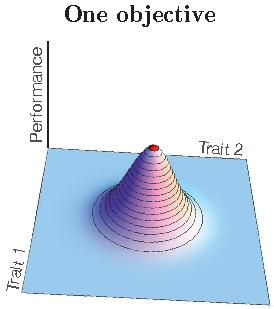
\includegraphics[width=\textwidth]{figures/objectivePerformance}
	\end{minipage}
	\textbf{b)}
	\hspace{0.2cm}
	\begin{minipage}[r]{0.40\textwidth}
		\centering
		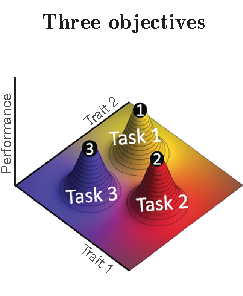
\includegraphics[width=\textwidth]{figures/objectivePerformance3}
	\end{minipage}
	\caption{\label{fig:objectivePerformance} \textbf{a)} Performance function of a single objective/task in trait-space (source: \cite{sheftel2013geometry}. \textbf{b)} Performance function of three objectives/tasks in trait-space. Archetypes are the local maxima (source: \cite{szekely2015mass}).}
\end{figure}

\begin{figure}[h]
\centering
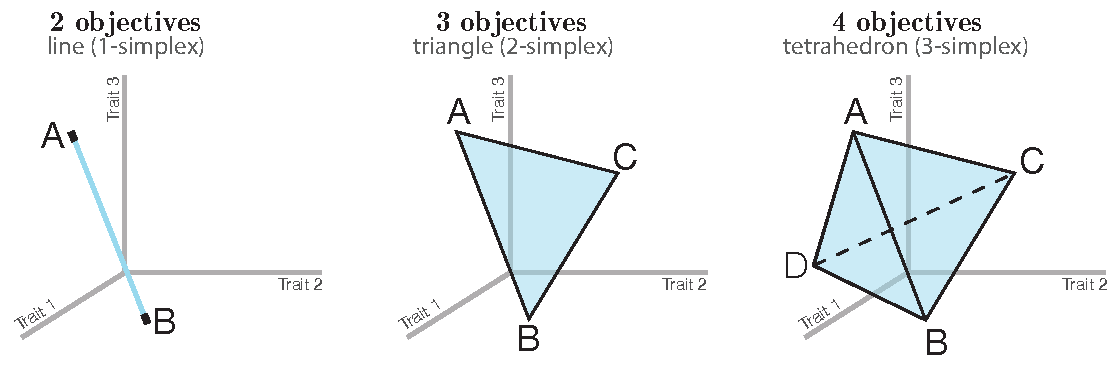
\includegraphics[width=\linewidth]{figures/paretoFronts} 
\caption{\label{fig:paretoFront} Pareto front regions (blue) for up to three objectives in trait-space. In the \textbf{2 objectives}-case the Pareto front spans the edge connecting objectives A and B. For \textbf{3 objectives} and \textbf{4 objectives} Pareto fronts are the area and volume, respectively, of the simplex spanned by the set of objectives.}
\end{figure}

\begin{figure}
	\centering
	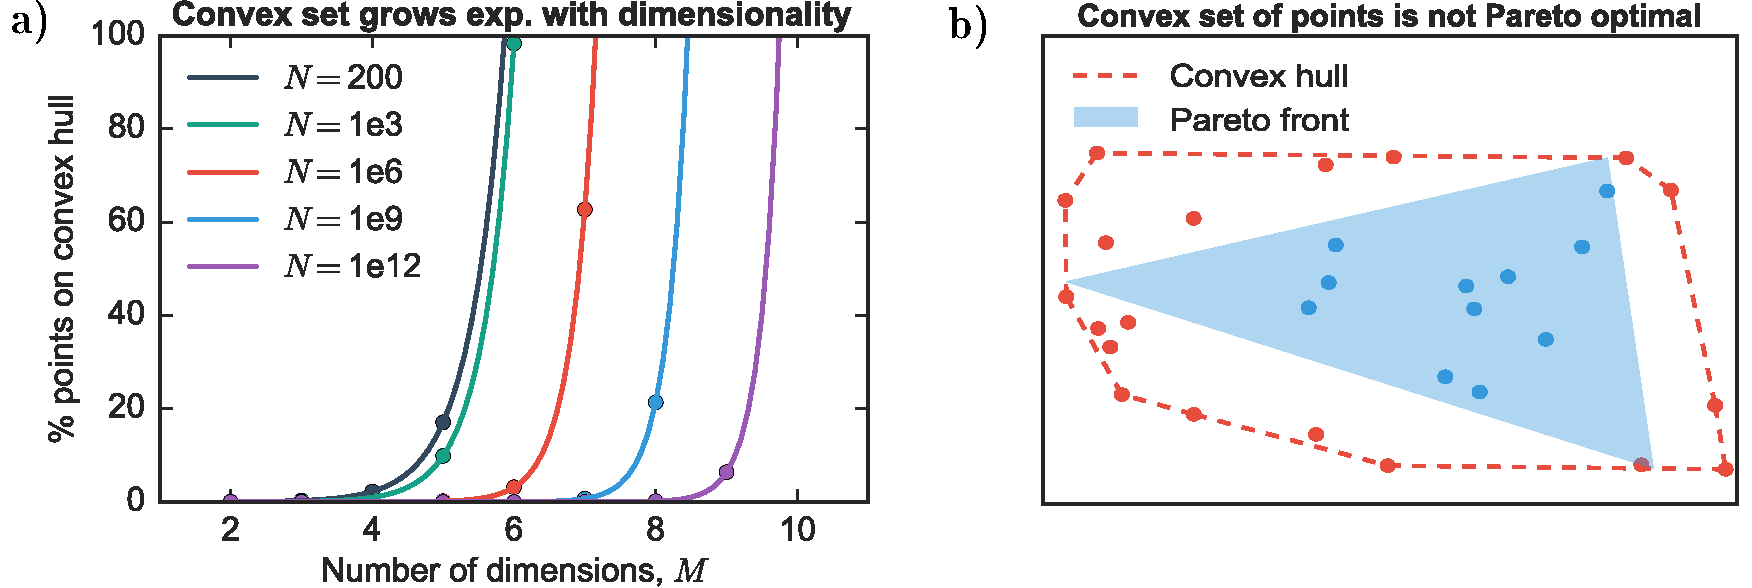
\includegraphics[width=1\textwidth]{figures/convexHullCurseOfDimensionality}
	\caption{\label{fig:convexHullCurseOfDimensionality} \textbf{a)} The size of the convex hull for $N$ points scale exponentially with the number of dimensions $M$ as $\mathcal{O}(\log{}n)^{M-1}$. Above five dimensions, many points are required in order to obtain a low ratio between the size of the convex set and the number of points. Note that the $M-$axis is discrete and that curves are plotted on a continuous scale for the sake of illustration. \textbf{b)} The Pareto front is a simplex anchored in $d+1$ points on the convex hull, and as such points on the hull that are not archetypes are not Pareto optimal.}
\end{figure}

\subparagraph*{The ParTI principle generalizes to any number of dimensions}
Since a triangle is just a special case of a $d$-simplex composed of $d+1$ vertices, the ParTI principle can be used to infer objectives in any number of dimensions. However, ParTI provides no "idiot-proof" solution to any dataset. For very high-dimensional data like gene expressions which may span a thousand dimensions, one shouldn't expect to find a thousand and one objectives. There is a purely mathematical reason for this. The convex set for any distribution of points grows exponentially with the number of dimensions as $\mathcal{O}(\log{(n)}^{M-1})$\mcite{morup2012archetypal}. Points on the convex hull are more likely to be outside of the Pareto front, and as such the possibility of finding valid simplex geometries (where \textit{valid} means that most points are on the Pareto front) in high-dimensional spaces is severely diminished. Figure \ref{fig:convexHullCurseOfDimensionality} illustrates that for over five dimensions, a very large number of datapoints are required to maintain a low ratio between the number of points in the convex set to the number of points in total.

Is this problematic? Somewhat yes, but recall from Section \ref{subsubsec:individualDifferencesAndPersonality} the concept of ESS. In most biological systems multiple ESSs can only exist alongside if they are frequency dependent and \textit{inter}-frequency dependent, and arguably there must be an upper limit to the number of complexly interacting strategies which can be ESS and exist alongside. That said, the above analysis cannot inform us about where this limit lies as biology has little regard for computational shortcomings.

\subparagraph*{Projections enable inference in high-dimensional data}
There is a solution to the problem pointed out above and illustrated in Figure \ref{fig:convexHullCurseOfDimensionality}. In high-dimensional systems such as cancer cells which are typically measured in terms of their gene expressions, objectives can be found using dimensionality reduction methods. In ParTI literature the prevailing such method is principle component analysis (PCA)\mcite{hart2015inferring}. PCA allows the analyst to project points in a high-dimensional space onto a subspace spanned an orthogonal basis of vectors which explain the most variance in the data. These vectors are called principle components (PC) and are computed as the eigenvectors of the covariance matrix. Informally, PCA can be thought of as casting a shadow of an object in such as way that the object can best be recognized. If the object was a sword, the first PC would follow the length of the sword and the second (being orthogonal to the first) would follow the guard and as such the best way to show that is was a sword just from looking at the shadow would be to project it onto these two components.

For objects that exist in high-dimensional spaces such as a point-cloud of gene expressions this method of "casting the shadow of highest explained variance" works methodically in exactly the same way as the sword example. Here, however, the analyst has more freedom to choose the dimensionality of the space projected to (the shadow). When ParTI treats high-dimensional data it looks for shadows that are shaped like simplexes (see Figure \ref{fig:paretoFront}}). For a low-dimensional projection where the points appear to fall inside a simplex, the vertices can be taken as the combinations of traits that allow for optimal performance of objectives, and each can in turn be identified by further analysis into how organisms with that combination of traits behave.